\documentclass{article}

\usepackage[english,polish]{babel} % Tutaj ważna jest kolejność atrybutów (dla pracy po polsku polish powinno być na końcu)
\usepackage{csquotes}
\usepackage{hyperref}
\usepackage{fancyhdr}
\usepackage{polski}
\usepackage{amsmath}
\usepackage{graphicx}
\usepackage{karnaugh-map}
\usepackage{parskip}
\usepackage{float}
\usepackage{geometry}
\usepackage{url}
\usepackage[
    backend=biber,
    style=numeric,
    sorting=ynt
]{biblatex}
\addbibresource{refs.bib}
\geometry{a4paper, margin=1in}
% \usepackage{tikzit}
% \input{res/style.tikzstyles}

% \input{style.tikzstyles}
%\lhead{\includegraphics[width=0.2\textwidth]{nyush-logo.pdf}}
\fancypagestyle{firstpage}{%
  \lhead{PWr}
  \chead{PSIM (Projekt)}
  \rhead{Zima 2024} 
}

%%%% PROJECT TITLE
\title{Wyjaśnialny system do klasyfikacji obrazów medycznych}

%%%% NAMES OF ALL THE STUDENTS INVOLVED (first-name last-name)
\author{\href{mailto:263917@student.pwr.edu.pl}{Michał Durkalec} - \texttt{263917@student.pwr.edu.pl}\\ 
        \href{mailto:263981@student.pwr.edu.pl}{Wiktoria Majewska} - \texttt{263981@student.pwr.edu.pl}}

\date{\vspace{-5ex}} %NO DATE

\begin{document}

\maketitle
\thispagestyle{firstpage}
\pagestyle{firstpage}

\section{Wstęp}
Celem projektu było opracowanie architektury systemu informatycznego, który pozwala na klasyfikację obrazów RTG klatki piersiowej z wykorzystaniem sieci neuronowych.
System ma wspierać lekarzy w~diagnostyce chorób poprzez automatyczną klasyfikację obrazów, a także dostarczać informacji o tym, jakie cechy obrazu zostały wykorzystane do podjęcia decyzji.

Głównym założeniem projektu nie jest stworzenie dokładnych modeli, ale eksploracja zagadnienia Explainable AI (XAI) \cite{gunning2019xai,barredoarrieta2020explainable} i możliwości implementacji mechanizmów XAI w aplikacjach dla użytkownika końcowego.

\subsection{Motywacja}
Zastosowanie głębokich sieci neuronowych w medycynie ma ogromny potencjał, ale wymaga specjalnych rozwiązań związanych z bezpieczeństwem i etyką.
W szczególności problematyczny jest brak zrozumienia mechanizmów decyzyjnych głębokich sieci neuronowych co generuje dalsze problemy regulacyjne i~etyczne. \cite{challen2019artificial}

Efektywne \emph{XAI} może pomóc w budowaniu zaufania i transparentości modeli dla użytkowników końcowych (pacjentów i lekarzy),
a co za tym idzie, znacząco przyspieszyć procesy diagnostyczne \cite{amann2020explainability}.
Ponadto wykorzystanie sieci głębokich w medycynie otwiera nowe możliwości w przygotowaniu spersonalizowanych planów terapii,
co może znacząco poprawić jakość życia pacjentów \cite{allen2024promise}.

\subsection{Zakres projektu}
Ze względu na ograniczenia czasowe projektu, zakres implementacji został znacząco zawężony, a głównym celem było przeanalizowanie możliwości i potrzeb użytkowników końcowych w zakresie wyjaśnialności modeli.
W szczególności w zakres projektu wchodziły następujące zagadnienia:
\begin{itemize}
  \item Architektura systemu informatycznego
  \item Proof-Of-Concept (PoC) dla klasyfikacji obrazów RTG klatki piersiowej
  \item Wizualizacja wyników klasyfikacji w końcowej aplikacji
  \item Analiza wyzwań związanych z wyjaśnialnością modeli
\end{itemize}

\section{Architektura systemu}
System oparty jest o architekturę klient-serwer, gdzie warstwa serwerowa odpowiada za przetwarzanie obrazów i klasyfikację, a warstwa klienta za interakcję z użytkownikiem.
Taki podział jest konieczny, ponieważ przetwarzanie obrazów i inferencja modeli wymaga dużej mocy obliczeniowej, a także specjalistycznych narzędzi i bibliotek.

\subsection{Warstwa klienta}
Prosta aplikacja webowa, która pozwala na przesłanie obrazu RTG klatki piersiowej i wyświetlenie wyniku klasyfikacji dla zalogowanych użytkowników.
W dlaszej perspektywnie aplikacja może zostać rozbudowana o dodatkowe funkcjonalności lub integrację z innymi systemami informatycznymi w placówce medycznej.

\textbf{Technologie:} React.js, TypeScript, Material-UI


\subsection{Warstwa serwera}
API REST, które pozwala na przesłanie obrazu RTG klatki piersiowej, przetworzenie go i zwrócenie wyniku klasyfikacji.
Serwer, w zależności od stopnia eksploatacji, może zostać zaimplementowany w~architekturze mikroserwisów, co pozwoli na łatwe skalowanie i zarządzanie zasobami.

\textbf{Technologie:} FastAPI, Python, PyTorch

\section{Proof-Of-Concept}
Proof-Of-Concept (PoC) został zaimplementowany w języku Python z wykorzystaniem biblioteki PyTorch. Kod źródłowy jest dostępny jako załącznik do raportu i może być uruchomiony na dowolnej maszynie z zainstalowanym środowiskiem Python i Jupyter.

Prototyp ilustruje, w jaki sposób można wykorzystać mechnizm Gradient CAM (Class Activation Mapping) \cite{selvaraju2017gradcam} do wizualizacji aktywacji w sieciach konwolucyjnych.
W ramach prototypu zrealizowano:
\begin{enumerate}
  \item Przygotowanie zbioru danych
  \item Dostosowanie modelu ResNet50 do klasyfikacji obrazów RTG klatki piersiowej
  \item Wizualizacja aktywacji w sieci
\end{enumerate}
Ze względu na ogranicznone możliwości obliczeniowe zaimplementowany model nie jest precyzyjny i nie nadaje się do zastosowań produkcyjnych;
jego głównym celem jest pokazanie możliwości wizualizacji aktywacji w sieciach konwolucyjnych.

\subsection{Zbiór danych}

Do treningu klasyfikatora wykorzystano zbiór danych oparty na \emph{CheXpert} \cite{irvin2019chexpert}.
Wykorzystany zbiór można pobrać z \url{https://www.kaggle.com/datasets/ashery/chexpert}.
Zbiór zawiera 224 316 obrazów RTG klatki piersiowej z 65 240 pacjentów, z których każdy został opisany przez 14 różnych etykiet.

\subsection{Model podstawowy}

Do klasyfikacji obrazów RTG klatki piersiowej wykorzystano zmodyfikowany model ResNet50 \cite{he2016deep}.
ResNet jest jednym z najpopularniejszych modeli w dziedzinie klasyfikacji obrazów i jest często wykorzystywany w zastosowaniach medycznych.
Ponadto ResNet jest dostępny w wielu różnych implementacjach w bibliotekach takich jak PyTorch czy TensorFlow.

\subsection{Dostosowanie modelu}

Model ResNet50 został dostosowany do klasyfikacji obrazów RTG klatki piersiowej poprzez zmianę warstwy wyjściowej.
ResNet jest modelem przeznaczonym do klasyfikacji obrazów z bazy ImageNet \cite{deng2009imagenet}, która zawiera obrazy z 1000 różnych klas.
W związku z tym, ostatnia w pełni połączona warstwa modelu ResNet50 została zastąpiona warstwą z 14 neuronami, odpowiadającymi 14 etykietom z CheXpert.

Następnie model był trenowany na zbiorze danych CheXpert przez 1 epokę z wykorzystaniem algorytmu \emph{AdamW} \cite{loshchilov2019decoupled}.
Jako funkcję straty wykorzystano \emph{BCEWithLogitsLoss}, a jako metrykę oceny jakości klasyfikacji \emph{AUROC} (Area Under Receiver Operating Characteristic).

Z powodu ograniczonych możliwości obliczeniowych nie podjęto próby usprawnienia modelu poprzez hiperparametryzację czy zastosowanie bardziej zaawansowanych technik regularyzacji.
Dostosowany model osiągnął jakość klasyfikacji na poziomie 0.5 AUROC, co jest wynikiem losowym i nie nadaje się do zastosowań produkcyjnych.

\subsection{Wizualizacja aktywacji}

Do wizualizacji aktywacji w wykorzystano mechanizm Gradient CAM (Class Activation Mapping) \cite{selvaraju2017gradcam}.
Pierwszym krokiem działania mechanizmu jest wybór ostatniej warstwy konwolucyjnej w modelu, która zawiera informacje o lokalizacji cech w obrazie.
Następnie obliczane są gradienty aktywacji względem klasy docelowej w tej warstwie, co pozwala na określenie, które obszary obrazu były najbardziej istotne dla klasyfikacji.
Obliczone gradienty są następnie agregowane w celu uzyskania mapy aktywacji, która jest nakładana na obraz wejściowy.

Do realizacji wizualizacji aktywacji wykorzystano biblioteki PyTorch, PIL.Image oraz pytorch\_gradcam.
W ramach prototypu możliwa jest wizualizacja aktywacji dla dowolnego obrazu RTG klatki piersiowej w~obrębie wszystkich 14stu klas dostępnych w zbiorze danych CheXpert.

Ponieważ prototyp jest oparty o model o niskiej jakości, wizualizacje aktywacji nie są wiarygodne i nie nadają się do zastosowań diagnostycznych.
Efektywnie, prototyp pokazuje jedynie w jaki sposób można zaimplementować mechanizm GradCAM w sieciach konwolucyjnych oraz jakiego rodzaju wyników należy oczekiwać i przetwarzać w warstwie prezentacji.

Mechanizm GradCAM został przetestowany również na bazowym modelu ResNet50, gdzie działał poprawnie, co potwierdza poprawność implementacji.
Brak satysfakcjonujących wyników (wizualizacji) w~PoC jest prawdopodobnie spowodowany niską precyzyjnością modelu.

\section{Wizualizacja warstwy prezentacji systemu}
Rysunki \ref{fig:start} i \ref{fig:results} przedstawiają wizualizację warstwy prezentacji systemu wykonaną za pomocą narzędzia Figma.

\begin{figure}[H]
  \centering
  \fbox{
    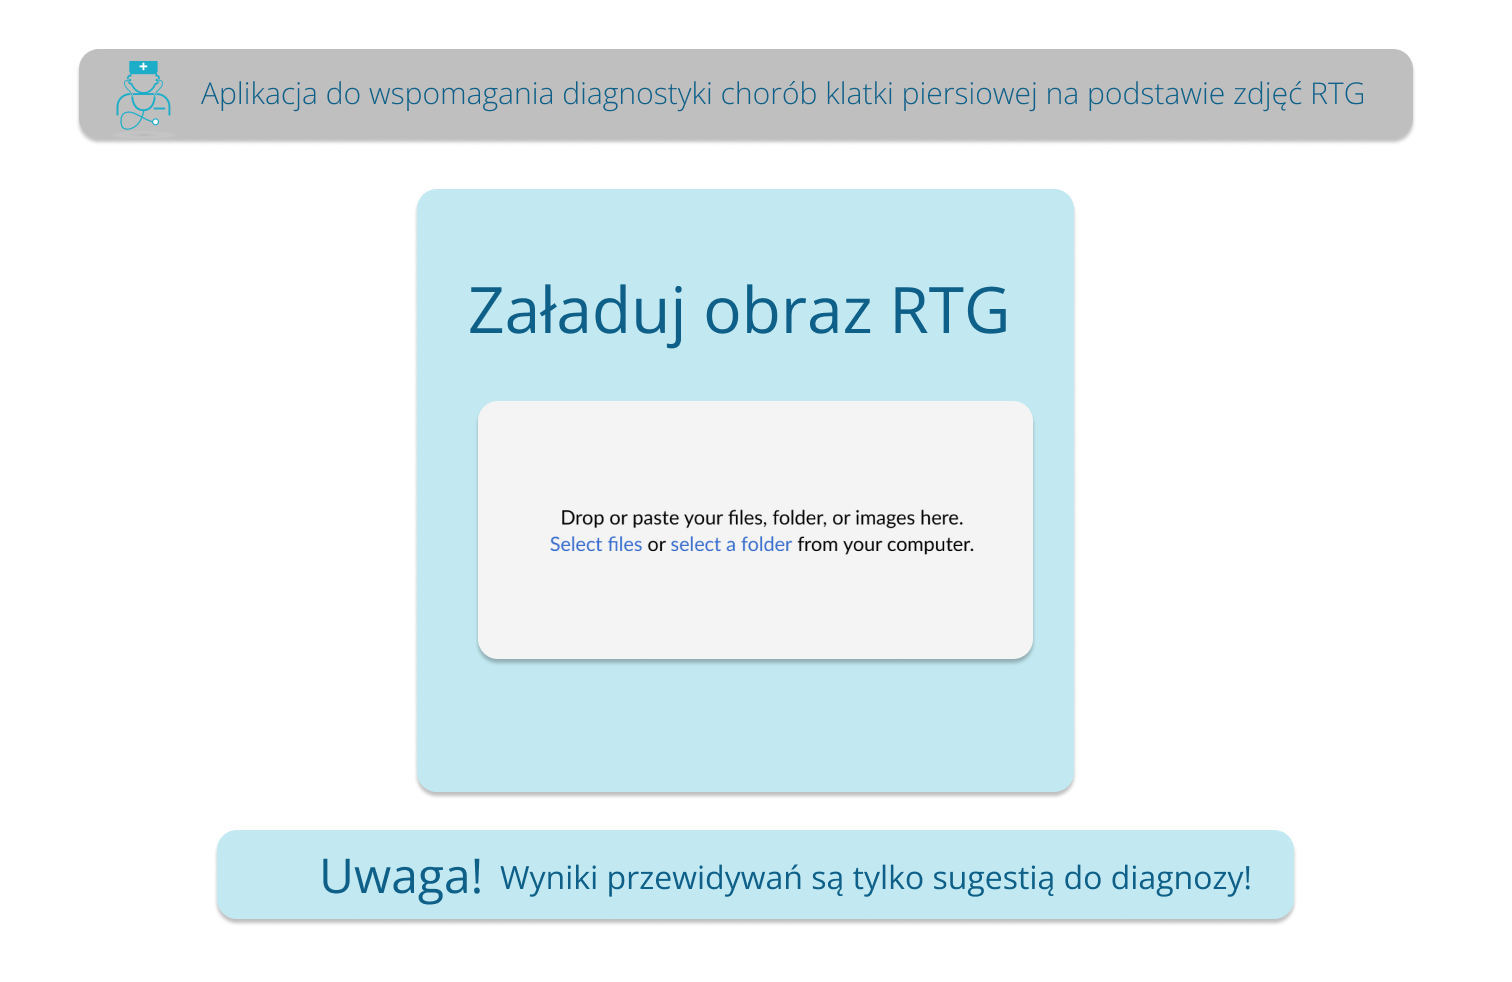
\includegraphics[width=\textwidth]{images/Widok startowy.png}
  }
  \caption{Ekran startowy aplikacji}
  \label{fig:start}
\end{figure}

\begin{figure}[H]
  \centering
  \fbox{
    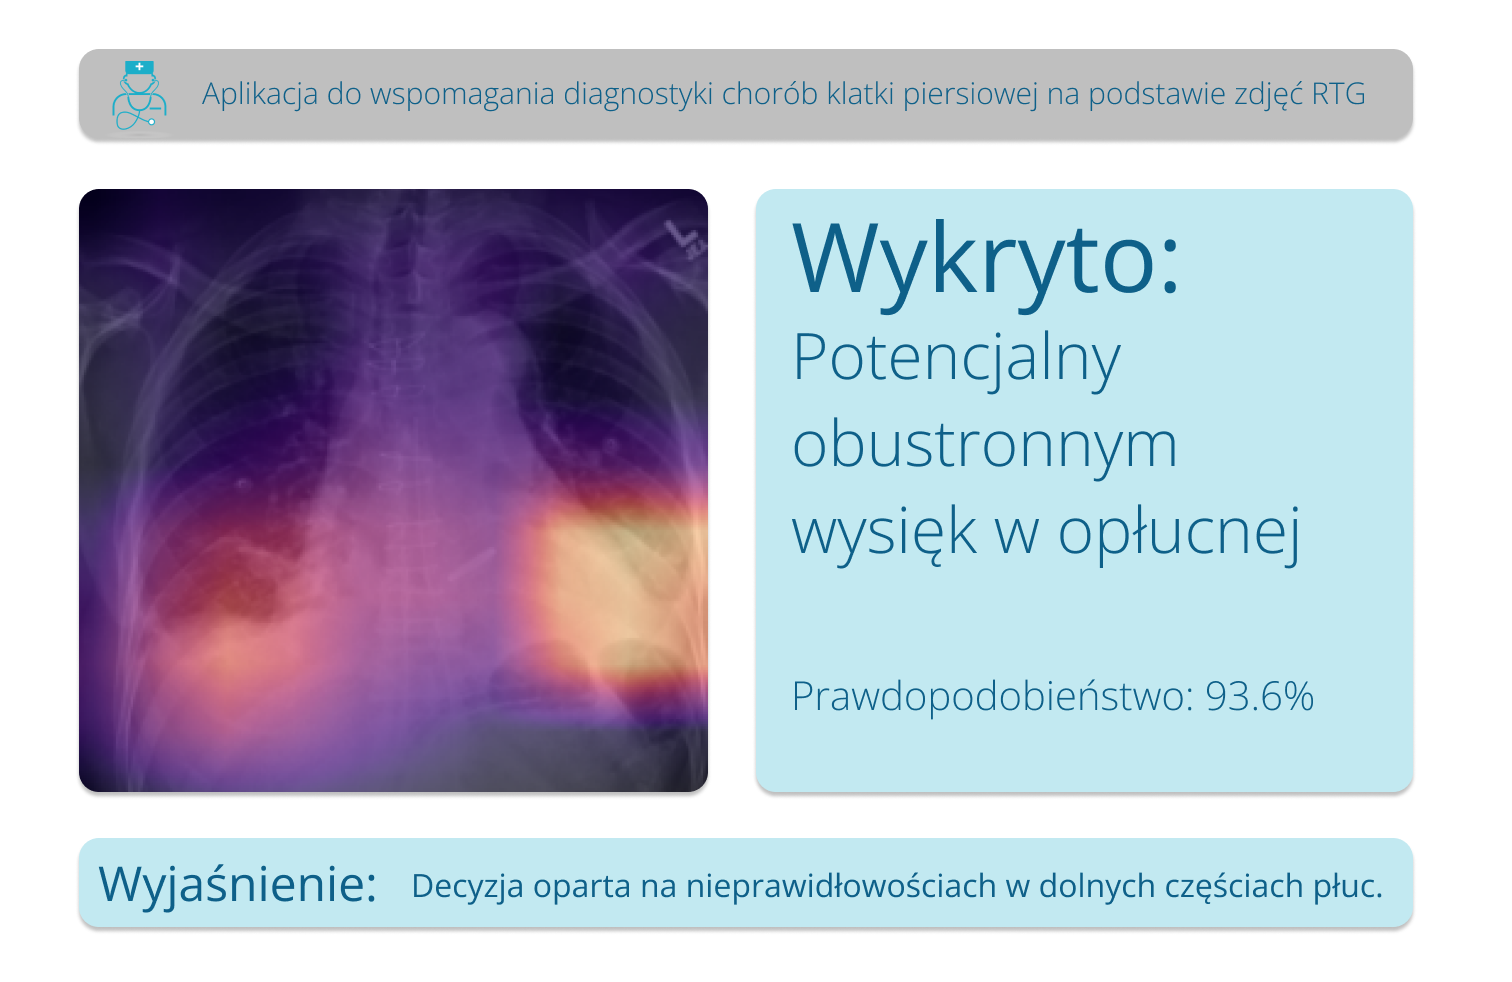
\includegraphics[width=\textwidth]{images/Wynik.png}
  }
  \caption{Ekran prezentacji wyników}
  \label{fig:results}
\end{figure}


\section{Analiza wyzwań związanych z wdrożeniem systemu}
Wprowadzenie aplikacji wspomagającej diagnostykę chorób klatki piersiowej z wykorzystaniem Explainable AI (XAI) wiąże się z istotnymi wyzwaniami etycznymi i prawnymi. Kluczowe obszary to:
\begin{itemize}
  \item \textbf{Ochrona danych medycznych przed nieautoryzowanym dostępem:} Dane medyczne są uznawane za szczególnie wrażliwe i wymagają najwyższego poziomu ochrony. Zgodnie z art. 9 ust. 1 RODO, przetwarzanie danych dotyczących zdrowia jest co do zasady zabronione, chyba że zachodzą określone wyjątki. W kontekście aplikacji mobilnej konieczne jest zapewnienie odpowiednich środków technicznych i organizacyjnych, aby chronić dane przed nieautoryzowanym dostępem, utratą czy modyfikacją.
  \item \textbf{Zgodność z RODO w przypadku przetwarzania danych osobowych:} RODO nakłada na administratorów danych obowiązek informowania pacjentów o celach i podstawach prawnych przetwarzania ich danych, a także o przysługujących im prawach. W przypadku aplikacji diagnostycznej konieczne jest spełnienie obowiązku informacyjnego wobec użytkowników oraz zapewnienie możliwości realizacji ich praw, takich jak prawo dostępu do danych czy ich sprostowania.
  \item \textbf{Ryzyko błędów klasyfikacji oraz wpływ takich błędów na decyzje diagnostyczne lekarzy:} Algorytmy AI mogą popełniać błędy, które w kontekście medycznym mogą prowadzić do poważnych konsekwencji dla pacjentów. Zgodnie z art. 4 ustawy o zawodach lekarza i lekarza dentysty, lekarz ma obowiązek wykonywać zawód zgodnie ze wskazaniami aktualnej wiedzy medycznej oraz z należytą starannością. Dlatego aplikacja powinna być traktowana jedynie jako narzędzie wspomagające, a ostateczna decyzja diagnostyczna powinna należeć do lekarza.
  \item \textbf{Transparentność działania modelu dzięki mechanizmom XAI:} Wykorzystanie mechanizmów XAI pozwala na wyjaśnienie decyzji podejmowanych przez model AI, co zwiększa zaufanie użytkowników do systemu. Transparentność działania algorytmu jest kluczowa, aby lekarze mogli zrozumieć podstawy decyzji i ocenić ich wiarygodność.
  \item \textbf{Ograniczenie aplikacji do narzędzia wspomagającego, a nie zastępującego lekarza w~procesie diagnozy:} Zgodnie z art. 37 ustawy o zawodach lekarza i lekarza dentysty, w razie wątpliwości diagnostycznych lekarz powinien zasięgnąć opinii właściwego specjalisty lub zorganizować konsylium lekarskie. Aplikacja powinna być traktowana jako wsparcie w procesie diagnostycznym, a nie jako zastępstwo dla profesjonalnej oceny medycznej. Lekarz ponosi odpowiedzialność za ostateczną diagnozę i leczenie pacjenta.
\end{itemize}

\section{Podsumowanie}

W ramach projektu, przeanalizowano możliwości zastosowania prostych mechanizmów XAI w aplikacjach medycznych.
Wdrożenie prostego systemu klasyfikacji obrazów medycznych z funkcją wizualizacji aktywacji nie jest wymagające technicznie, ale wiąże się z istotnymi wyzwaniami etycznymi i prawnymi.
System o proponowanej architekturze nadaje się do wdrożenia w środowisku produkcyjnym, ale wymaga znaczącego rozwoju w zakresie jakości modeli.
Ponadto, w ramach projektu nie zostały rozważone wymagania związane z bezpieczeństwem i niezawodnością systemu, które są kluczowe w zastosowaniach medycznych.

W obecnym środowisku regulacyjnym modele AI w medycynie, nawet stosujące techniki XAI, nie mogą zastępować decyzji lekarzy.
System może służyć jedynie jako narzędzie wspomagające, które dostarcza informacji o procesie decyzyjnym modelu, ale ostateczna decyzja diagnostyczna musi zostać podjęta przez radiologa.

\newpage
\printbibliography

\end{document}